\chapter{Interview mit Kathrin Favero vom \acs{bag}}
\authortoc{\bastian}{\chapterident}
Wir haben das BAG angerufen und nachgefragt, ob wir mit ihnen ein Interview führen können. Darauf verwies uns eine Mitarbeiterin auf eine Informationsmail namens “media@bag.admin.ch”. An diese Mail haben wir alle Fragen geschickt. Eine Woche später erhielten wir eine ausführliche Antwort des BAG. Nachfolgend präsentieren wir unser Interview:
\section{Kernpunkte eines gesunden Lebensstils}
Wir haben das BAG gefragt, was ihrer Meinung nach die Kernpunkte eines gesunden Lebensstils sind. Darauf antworteten sie kurz und knackig, dass für sie Achtsamkeit, Freude an dem, was man tut, ausreichend Bewegung, ausgewogene
Ernährung, kein Tabak und wenig Alkohol als wichtige Träger für einen gesunden Lebensstils gelten.
\section{Unsere Unterteilung des Themas}
Unser Thema haben wir in 5 Gruppen aufgeteilt: Ernährung, Bewegung, Schlaf, Gewohnheiten und Zeitmanagement. Nun wollten wir vom BAG wissen, was sie von unserer Gliederung halten. Das \acs{bag} meinte dazu, dass es schon sehr gut durchdacht ist und ergänzte bei den Gewohnheiten noch folgendes “Bei den Gewohnheiten versucht man mit der Verhaltensökonomie die «gesunde Wahl» zu erleichtern, d. h. z. B. beim gewohnten Weg zum Schulzimmer die Wahl zur Benutzung der Treppe zu erleichtern, in dem vor Ort, im Moment der Entscheidung, ein Hinweis (Poster, Tafel, Treppen Verschönerung, etc) erscheint, der einem bewusst macht, dass man die Treppe anstelle des Lifts nehmen soll.” Damit meinen sie, dass man die Gewohnheit steuern und sich so für die gesündere Variante entscheiden kann. Zudem fehlt dem BAG das Soziale, welches der psychischen Gesundheit sehr gut tut, wie z. B. Freunde, Austausch, Spiel und Freude.
In Bezug auf das Soziale kam das Thema mit der Definition der WHO auf: “Die Gesundheit ist ein Zustand des vollständigen körperlichen, geistigen und sozialen Wohlergehens und nicht nur das Fehlen von Krankheit oder Gebrechen.” \cite{gesundheit_definition}
https://de.wikipedia.org/wiki/Gesundheit
Laut \acs{bag} hat die WHO bei dieser Definition auch an das Soziale gedacht. Damit wird gemeint, dass zum Beispiel im Bereich strukturelle Bewegungsförderung (Förderung von körperlicher Aktivität über das gebaute Umfeld wie z. B. Fussgänger- und Velowege) darauf geachtet wird, dass bei der Quartiergestaltung das soziale Leben auch gefördert wird. Dies hat einen positiven Einfluss auf die Psyche der Anwohner. Ebenfalls ist es auch eine Motivation für mehr Bewegung, da man sich dadurch in einer schönen, naturnahen und sicheren Umgebung aufhalten kann und dabei vielleicht auch noch Menschen antrifft.
\section{Rolle der Ernährung}
Die Frage lautete, was für eine Rolle die Ernährung bei einem gesunden Lebensstil hat. Dabei konnte uns das \acs{bag} nicht gross weiterhelfen, jedoch verwiesen sie uns zu einer anderen Fachstelle. Dabei haben sie uns eine Ansprechpartnerin des  Bundesamt für Lebensmittelsicherheit und Veterinärwesen gegeben. Leider konnten wir sie aber nicht befragen. Ebenfalls hat uns das \acs{bag} eine Webseite angegeben, auf der man sich nochmals gründlich in Bezug auf Ernährung informieren kann.
\newline
\url{https://www.sge-ssn.ch/}
\section{Probleme bei ungesunder Ernährung}
Wir stellten dem \acs{bag} die Frage, was für Probleme ein ungesunder Lebensstil mit sich bringt. Ihre Antwort darauf war, dass es kurzfristig nicht bemerkbar sei, jedoch gibt es über einen längeren Zeitraum grosse Probleme. So kann man übergewichtig werden, Herz-Kreislauf Erkrankungen und Diabetes bekommen, bis hin zum frühzeitigen Tod. Für mehr Informationen verwiesen sie uns auf folgende Webseite: 
\newline
\url{https://www.bag.admin.ch/bag/de/home/strategie-und-politik/nationale-gesundheitsstrategien/strategie-nicht-uebertragbare-krankheiten.html}
\section{Benötigte Bewegung}
Als Nächstes haben wir dem \acs{bag} die Fragen gestellt, wieviel Bewegung man braucht und was für eine Art von Bewegung sie uns empfehlen. Dabei sagten sie, dass die Bewegungsempfehlung je nach Bevölkerungsgruppe unterschiedlich sei. Für eine genaue Empfehlung haben sie uns auf folgende Seite verwiesen:
\newline
\url{https://www.bag.admin.ch/bag/de/home/gesund-leben/gesundheitsfoerderung-und-praevention/bewegungsfoerderung/bewegungsempfehlungen.html}
\newline
Auf dieser Seite sind sämtliche Informationen zur Bewegungsempfehlung rund um die Altersgruppen. 
\section{Definition und individuelle Ansicht}
Unsere Fragestellung lautete, ob es für das \acs{bag} eine Definition von “Gesund” gibt und wie sehr diese abhängig von Person zu Person ist. Bei der Definition verwiesen sie uns auf die Definition des WHO “Die Gesundheit ist ein Zustand des vollständigen körperlichen, geistigen und sozialen Wohlergehens und nicht nur das Fehlen von Krankheit oder Gebrechen.” \cite{gesundheit_definition}
In Bezug auf die Abhängigkeit zwischen verschiedenen Personen gaben sie uns die Auskunft, dass die eigene Wahrnehmung je nach Person individuell und ganz anders wahrgenommen wird. Was das \acs{bag} jedoch beobachtet hat, ist, dass sich ältere Personen in der Schweiz häufig noch sehr gesund fühlen. Der Zusammenhang besteht darin, dass die ältere Altersklasse sich gegenseitig untereinander und nicht mit jüngeren Personen vergleichen. Ebenfalls haben sie uns einen Artikel mitgeliefert, welcher sich auf die Selbstwahrnehmung der Schweizer Bevölkerung und deren Gesundheitszustand bezieht. Folgend der Link dazu:
\newline
\url{https://www.bfs.admin.ch/bfs/de/home/statistiken/querschnittsthemen/wohlfahrtsmessung/wohlfahrt/gesundheit/gesundheitszustand.html}
\section{Unterschiede der Altersgruppe}
Dem \acs{bag} haben wir die Frage gestellt, ob es Unterschiede zwischen verschiedenen Altersgruppen gibt und wenn ja, ob sie dazu ein paar Beispiele hätten. Hierbei hat sich das \acs{bag} auf die Jugend und deren Entwicklung bis zum Erwachsensein bezogen. Zitat \acs{bag}: “Ja, z. B. ist das Gehirn in der Jugend immer noch in Entwicklung. Auf der einen Seite entwickeln sich wichtige Fähigkeiten wie die Kontrolle von Emotionen (es ist nicht nur ein Lernprozess, sondern das Gehirn entwickelt physiologisch den Teil, welchen es dazu braucht). Auf der anderen Seite ist ihr Gehirn empfindlicher auf psychoaktive Substanzen und trägt eher Schäden davon als das Gehirn von erwachsenen Personen.” Damit spricht es zugleich auch der Konsum von Suchtmitteln, Drogen und Alkohol an. Dieser kann in jungen Jahren noch Schäden in der Entwicklung hervorrufen, welche diverse Folgen haben könnten.
\section{Gesunder Lebensstil in jungen Jahren}
Wir haben das \acs{bag} gefragt, wieso ein gesunder Lebensstil in jungen Jahren (Kind/Jugendlicher) schon wichtig ist. Darauf gaben sie uns die Antwort, dass es wichtig ist, dass sich die Kinder und Jugendlichen gesund ernähren und Sport treiben. Der Grund dafür ist, dass man in diesem Alter Gewohnheiten schnell annimmt und wenn gute Erfahrungen gemacht werden, werden diese auch weitergeführt. In Zukunft werden diese positiven Einflüsse, sei es im Sport oder der Ernährung, unbewusst ein Teil dieser Person sein. Das heisst sie wird automatisch Sport machen wollen oder auch gesünder essen wollen.
\pagebreak
\section{Gesunde Gesellschaft}
Unsere Frage lautete, ob das \acs{bag} die Lebensweise der Bevölkerung als gesund einstuft oder nicht. Darauf konnten sie leider keine Antwort liefern. Wir konnten jedoch mit eigenen Recherchen herausfinden, dass die Gesundheit der Schweizer Bevölkerung (Stand 2017) in einem relativ guten Zustand ist. Im Anschluss der Link zu der Seite mit allen weiteren Informationen zu diesem Thema.
\begin{figure}[H]
  \centering
  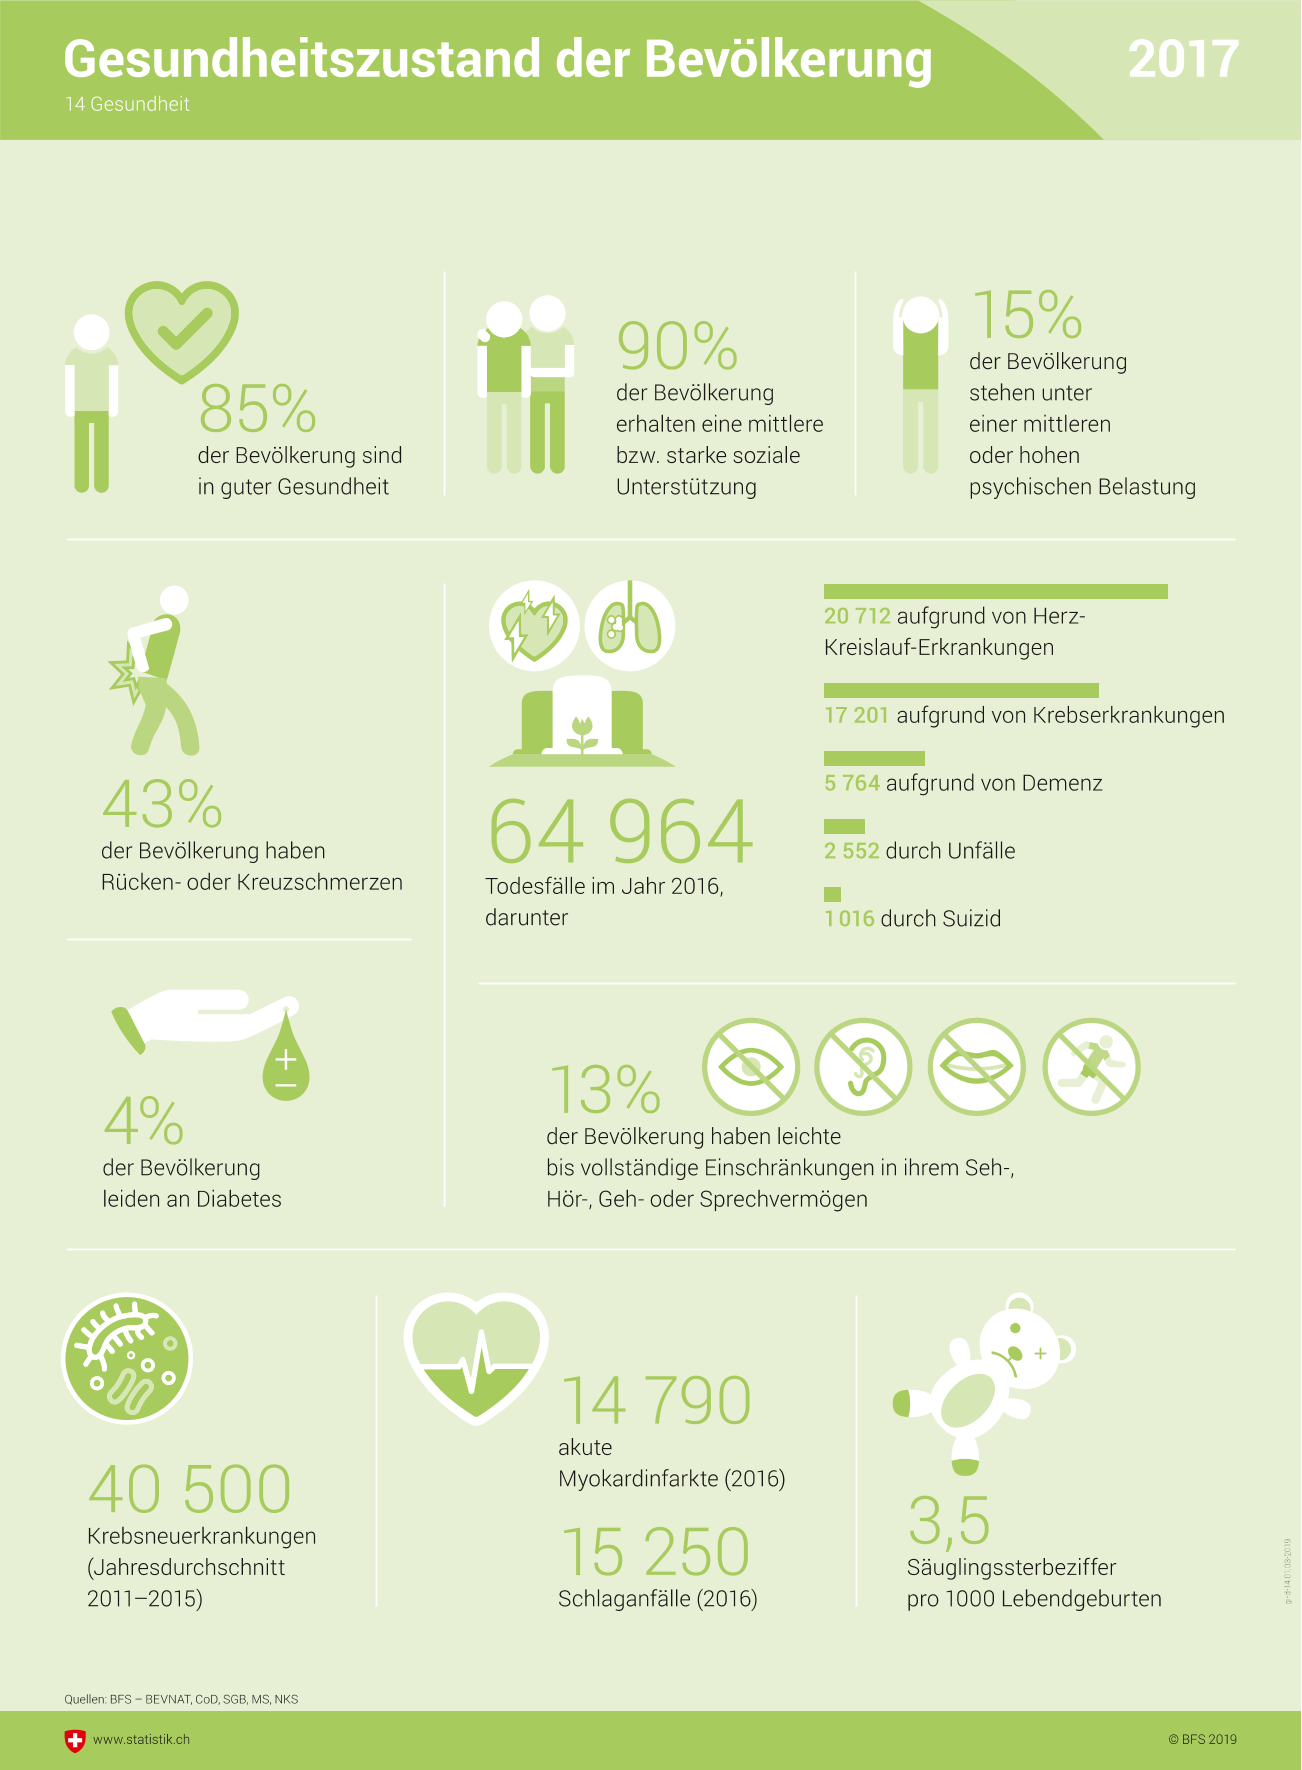
\includegraphics[width=0.75\linewidth]{./images/gesundheitszustand_der_bevoelkerung.png}
  \caption{Gesundheitszustand der Schweizer Bevölkerung}
  \label{fig:gesundheitszustand}
  \captionsetup{font={footnotesize}}
  \caption*{\url{https://www.bfs.admin.ch/bfs/de/home/statistiken/gesundheit/gesundheitszustand.html}}
\end{figure}
\section{Unternehmungen des \acsp{bag} und deren Kampagnen}
Zuletzt haben wir das \acs{bag} gefragt, was es alles für die Gesundheit der Bevölkerung unternimmt und was es für Kampagnen dazu gibt. Darauf lautete die Antwort, dass alles, was das \acs{bag} tut, der Gesundheit der Bevölkerung nutzen soll. Dabei zeigten sie uns einige Links auf, welche die Gesundheitsförderung oder auch die Sucht thematisieren. Nachfolgend die Links zu den Informationsseiten: 
\begin{itemize}
  \item \textbf{Gesundheitsförderung \& Prävention}
  \newline
  \url{https://www.bag.admin.ch/bag/de/home/gesund-leben/gesundheitsfoerderung-und-praevention.html}
  \item \textbf{Sucht \& Gesundheit}
  \newline
  \url{https://www.bag.admin.ch/bag/de/home/gesund-leben/sucht-und-gesundheit.html}
\end{itemize}
Auf die Anfrage bezüglich der Kampagnen haben sie uns ebenfalls einige Informationsseiten mit diversen Kampagnen geschickt. Aktuell haben sie eine Kampagne am Laufen, welche sich mit dem ständigen Sitzen befasst und einem dazu ermuntert, immer wieder zu stehen. Der Link zu der Kampagne lautet:
\newline
\url{https://www.bag.admin.ch/bag/de/home/gesund-leben/gesundheitsfoerderung-und-praevention/bewegungsfoerderung/auf-stehen.html}
\newline
Ebenfalls haben sie zwei abgeschlossene Kampagnen. Zum einen die Alkoholprävention und zum anderen die Tabakprävention:
\begin{itemize}
  \item \textbf{Alkoholprävention (abgeschlossene Kampagne)}
  \newline
  \url{https://www.bag.admin.ch/bag/de/home/strategie-und-politik/kampagnen/alkoholpraeventionskampagne.html}
  \item \textbf{Tabakprävention (abschlossene Kampagne)}
  \newline
  \url{https://www.bag.admin.ch/bag/de/home/strategie-und-politik/kampagnen/tabakpraeventionskampagne.html}
\end{itemize}
\vspace{50pt}
\textbf{\textit{Das Interview mit den Original-Fragen sowie Antworten ist im Anhang zu finden.}}